\chapter{Perturbation, Chaos, And Celestial Mechanics}
\label{chap:perturbation-chaos}

\section{What This Chapter Studies}
\label{sec:perturbation-chapter-purpose}

The central example is a massless asteroid perturbed by Jupiter while orbiting
the Sun. The unperturbed problem is Kepler motion, one of the most integrable
systems in classical mechanics. The perturbation introduces resonances, broken
invariant tori, chaotic transport, and possible ejection.

\begin{assumption}[Restricted planar model]
Unless otherwise stated, this chapter uses a planar restricted model:
\begin{enumerate}
\item the Sun has mass \(M_\odot\);
\item Jupiter has mass \(M_J\) and follows a prescribed circular orbit;
\item asteroids are massless test particles;
\item asteroid-asteroid interactions are neglected;
\item all motion is confined to one plane.
\end{enumerate}
This model is not a high-precision Solar System ephemeris. It is a controlled
Hamiltonian laboratory for perturbation, resonance, and transport.
\end{assumption}

\begin{table}[htbp]
\centering
\caption{Notation for perturbation theory, KAM, and the restricted
Sun-Jupiter-asteroid model.}
\label{tab:perturbation-chaos-notation}
\small
\begin{tabular}{p{0.18\textwidth}p{0.48\textwidth}p{0.25\textwidth}}
\toprule
Symbol & Meaning & Units in demos\\
\midrule
\(G\) & gravitational constant & \(4\pi^2\) in AU, yr, solar masses\\
\(M_\odot\) & solar mass & \(1\)\\
\(M_J\) & Jupiter mass & \(9.543\times 10^{-4}M_\odot\)\\
\(r,v,p\) & asteroid position, velocity, canonical momentum & AU, AU/yr, mass-scaled\\
\(h\) & specific Kepler Hamiltonian & energy per unit mass\\
\(\mu\) & reduced mass in two-body problem & mass\\
\(\ell\) & angular momentum per unit mass & AU\(^2\)/yr\\
\(a\) & asteroid semimajor axis & AU\\
\(a_J\) & Jupiter semimajor axis & AU\\
\(e,\varpi\) & eccentricity and longitude of periapse & dimensionless, radians\\
\(n\) & asteroid mean motion & rad/yr\\
\(n_J\) & Jupiter mean motion & rad/yr\\
\(\eps\) & perturbation strength & often proportional to \(M_J/M_\odot\)\\
\((I,\theta)\) & action-angle coordinates & \(I\in U,\theta\in\mathbb T^N\)\\
\(H_0,H_1\) & integrable Hamiltonian and perturbation & model dependent\\
\(\omega_0(I)\) & unperturbed frequency vector & rad/time\\
\(k\) & integer Fourier/resonance vector & element of \(\Z^N\)\\
\(S_1\) & first generating-function correction & canonical perturbation theory\\
\(H_{1k}\) & \(k\)-th Fourier coefficient of \(H_1\) & same units as \(H\)\\
\(\alpha,\tau\) & Diophantine constants & lower-bound parameters\\
\(K\) & standard-map kick strength & dimensionless\\
\(T_K,\Psi\) & standard map or other area-preserving map & discrete-time map\\
\(N,T,\Delta t\) & sample count, integration horizon, time step & demo parameters\\
\(\widehat P_{\mathrm{ej}}\) & finite-time ejection-probability estimate & dimensionless\\
\bottomrule
\end{tabular}
\end{table}

\paragraph{Roadmap.}
The chapter begins with the Kepler problem because perturbation theory needs an
integrable reference system. It then introduces resonances, small divisors, and
Diophantine conditions, which explain why some invariant tori are robust while
others are fragile. The KAM theorem gives the positive result: many sufficiently
irrational tori persist under small perturbation. The Poincare-map and
standard-map sections show the complementary phenomenon: resonant tori break
into islands and chaotic layers. The restricted Sun-Jupiter-asteroid model then
turns this geometry into a numerical ejection experiment.

There are three levels of description to keep separate. The analytic level asks
whether a formal canonical transformation can remove angle dependence. The
geometric level asks which invariant tori, islands, and separatrices organize
phase space. The numerical level asks how an ensemble moves through that
geometry over a finite time. The asteroid ejection probability belongs to the
third level, but it is meaningful only because the first two levels explain
where transport channels come from.

\paragraph{How approximations are labelled.}
Perturbation theory is useful only when the bookkeeping is explicit. In this
chapter \(H_0\) denotes the exactly integrable reference problem, \(\eps H_1\)
denotes a controlled perturbation, \(O(\eps^2)\) denotes terms dropped by a
first-order calculation, and resonance conditions such as \(k\cdot\omega=0\)
identify where that first-order calculation is least trustworthy. Numerical
experiments later in the chapter do not replace these estimates; they test the
transport suggested by them over a stated finite time horizon.

\section{The Kepler Problem}
\label{sec:kepler-perturbation}

For two bodies of masses \(m_1,m_2\), let
\[
  r=x_1-x_2
\]
be the relative position and
\[
  \mu=\frac{m_1m_2}{m_1+m_2}
\]
the reduced mass. The relative Hamiltonian is
\[
  H(r,p)=\frac{\norm{p}^2}{2\mu}-\frac{Gm_1m_2}{\norm r}.
\]
For a massless asteroid around the Sun, one usually divides by asteroid mass and
works with the specific Hamiltonian
\[
  h(r,v)=\frac12\norm v^2-\frac{GM_\odot}{r},
  \qquad r=\norm r.
\]

\begin{derivation}[Kepler orbit equation]
The angular momentum per unit mass is
\[
  \ell=r^2\dot\theta.
\]
This \(\ell\) is the specific angular momentum. In
Chapter~\ref{chap:lag-ham}, the two-body Kepler derivation used the massful
angular momentum \(\ell_{\mathrm{mass}}=\mu r^2\dot\theta\); the two symbols
differ by the reduced mass because this chapter has divided the Hamiltonian by
the asteroid mass. Section~\ref{subsec:detailed-binet} gives the same Binet
equation with an arbitrary particle mass \(m\); setting \(m=1\) gives the
specific convention used here.
For a central potential, \(\ell\) is conserved. The radial equation is
\[
  \ddot r-r\dot\theta^2=-\frac{GM_\odot}{r^2}.
\]
Set \(u=1/r\). Using
\[
  \frac{\dd}{\dd t}=\dot\theta\frac{\dd}{\dd\theta}
  =
  \ell u^2\frac{\dd}{\dd\theta},
\]
the radial equation loses its explicit time dependence and becomes Binet's
equation for the orbit shape:
\[
  \frac{\dd^2u}{\dd\theta^2}+u=\frac{GM_\odot}{\ell^2}.
\]
Therefore
\[
  u(\theta)=\frac{GM_\odot}{\ell^2}\left(1+e\cos(\theta-\varpi)\right),
\]
or
\[
  \boxed{
  r(\theta)=\frac{a(1-e^2)}{1+e\cos(\theta-\varpi)}
  }.
\]
Here \(a\) is the semimajor axis, \(e\) is eccentricity, and \(\varpi\) is the
longitude of periapse.
\end{derivation}

Bound Kepler orbits have energy
\[
  h=-\frac{GM_\odot}{2a}.
\]
Kepler's third law follows from the period \(T\):
\[
  n^2a^3=GM_\odot,\qquad n=\frac{2\pi}{T}.
\]

\section{Action-Angle View Of Kepler Motion}
\label{sec:kepler-action-angle}

The Kepler problem is more than solvable; it is superintegrable. For
perturbation theory, the most useful idea is that unperturbed motion can be
written in action-angle form:
\[
  H_0=H_0(I),
  \qquad
  \dot I=0,
  \qquad
  \dot\theta=\omega(I).
\]
For a near-integrable Hamiltonian,
\[
  H(I,\theta)=H_0(I)+\eps H_1(I,\theta),
\]
the actions are no longer exactly constant:
\[
  \dot I=-\eps\frac{\partial H_1}{\partial \theta},
  \qquad
  \dot\theta=\frac{\partial H_0}{\partial I}
  +
  \eps\frac{\partial H_1}{\partial I}.
\]
The small parameter \(\eps\) should be interpreted physically. In the
Sun-Jupiter-asteroid problem, a natural scale is \(M_J/M_\odot\), though close
encounters and resonances can amplify its effect.

\section{Resonance}
\label{sec:resonance}

\begin{definition}[Resonance]
A resonance occurs when there is a nonzero integer vector \(k\in\Z^n\) such
that
\[
  k\cdot\omega(I)=0.
\]
Near resonance, phase combinations that normally average out become slow and
can accumulate over long times.
\end{definition}

For mean-motion resonance with Jupiter, a \(p:q\) resonance means
\[
  \frac{n}{n_J}\approx \frac{p}{q}.
\]
Using Kepler's law,
\[
  \frac{n}{n_J}\approx
  \left(\frac{a_J}{a}\right)^{3/2},
\]
so the nominal resonance location is
\[
  \boxed{
  a_{p:q}=a_J\left(\frac{q}{p}\right)^{2/3}
  }.
\]
This formula is only the center of a resonance zone. The width of the zone
depends on the perturbation strength, eccentricity, and the order of the
resonance. The point of marking the nominal location is to identify where slow
angle combinations can form; the later chaos discussion explains what happens
inside and near those zones.

\begin{figure}[htbp]
\centering
\begin{tikzpicture}[x=0.72cm,y=1cm, >=Latex]
  \draw[->] (0,0) -- (13.8,0) node[right] {\(a\) [AU]};
  \foreach \x/\lab in {0/2.0,2/2.5,4/3.0,6/3.5,8/4.0,10/4.5,12/5.0}
    \draw (\x,0.07) -- (\x,-0.07) node[below] {\lab};
  \draw[ultra thick, blue!35] (0.1,0) -- (7.0,0);
  \node[blue!60!black] at (3.6,0.45) {asteroid-belt-like annulus};
  \foreach \x/\lab in {2.008/3:1,3.302/5:2,3.833/7:3,5.114/2:1}
  {
    \draw[red, thick] (\x,-0.55) -- (\x,0.9);
    \node[red, rotate=90, anchor=south] at (\x,0.95) {\lab};
  }
  \fill[orange!80!black] (12.82,0) circle (2.2pt);
  \node[orange!80!black, above] at (12.82,0.12) {Jupiter};
\end{tikzpicture}
\caption{Nominal mean-motion resonance locations with Jupiter, shown
across an asteroid-belt-like range. The resonance positions use
\(a_{p:q}=a_J(q/p)^{2/3}\); the figure now includes Jupiter's orbital radius to
show that the listed resonances lie interior to Jupiter.}
\label{fig:jupiter-resonance-locations}
\end{figure}

\section{Perturbing An Integrable System}
\label{sec:perturbing-integrable-system}

The central perturbation question is the following. Suppose the unperturbed
Hamiltonian is integrable and has action-angle coordinates:
\[
  H_0=H_0(I),
  \qquad
  (I,\theta)\in U\times\mathbb T^N,
  \qquad
  \dot I=0,\quad \dot\theta=\omega_0(I),
\]
where
\[
  \omega_0(I)=\frac{\partial H_0}{\partial I}.
\]
Now add a small generic perturbation:
\[
  H(I,\theta)=H_0(I)+\eps H_1(I,\theta),
  \qquad
  0<\eps\ll 1.
\]
What happens to the invariant tori \(I=\text{constant}\)?

Historically, two tempting answers were both too simple. One might hope that
the perturbed system is still integrable after a clever change of variables.
One might also expect that a generic perturbation destroys the tori and makes a
typical orbit wander ergodically through the available energy surface. KAM
theory gives the subtler answer: for small analytic perturbations, most
sufficiently irrational tori persist, while resonant regions create islands,
separatrices, and chaotic transport.

The historical landmarks are the Fermi-Pasta-Ulam-Tsingou numerical experiment
of 1953, which contradicted naive ergodicity, and the
Kolmogorov-Arnold-Moser work from roughly 1954--1963, which explained why
small perturbations can leave most invariant tori intact while still allowing
chaotic regions.

\section{Canonical Perturbation Theory And Small Divisors}
\label{sec:canonical-perturbation-small-divisors}

We first ask whether a canonical transformation can remove the angle dependence
order by order. Use a type-II generating function
\[
  S(I',\theta)=I'\cdot\theta+\eps S_1(I',\theta)+\eps^2S_2+\cdots.
\]
The transformation is
\[
  I_i=\frac{\partial S}{\partial \theta^i},
  \qquad
  \theta'^i=\frac{\partial S}{\partial I'_i}.
\]
To first order,
\[
  I=I'+\eps\frac{\partial S_1}{\partial \theta}+O(\eps^2).
\]
If the transformed Hamiltonian is angle-independent to order \(\eps\),
\[
  H'(I')=H(I,\theta),
\]
then expanding gives
\[
  H'(I')
  =
  H_0(I')
  +
  \eps\left[
    \omega_0(I')\cdot\frac{\partial S_1}{\partial \theta}
    +
    H_1(I',\theta)
  \right]
  +
  O(\eps^2).
\]
Thus we need
\[
  \omega_0(I')\cdot\frac{\partial S_1}{\partial \theta}
  =
  f_1(I')-H_1(I',\theta),
\]
where \(f_1(I')\) will become the first correction to the new Hamiltonian.
Since \(S_1\) must be periodic in each angle, the average over the torus of the
left side is zero. Therefore
\[
  f_1(I')=\langle H_1(I',\theta)\rangle_\theta.
\]

Expand the perturbation in Fourier modes:
\[
  H_1(I,\theta)=\sum_{k\in\Z^N} H_{1k}(I)e^{ik\cdot\theta}.
\]
The \(k=0\) mode is the average. For \(k\neq0\), the homological equation gives
\[
  i(k\cdot\omega_0(I'))S_{1k}(I')=-H_{1k}(I'),
\]
or
\[
  \boxed{
  S_{1k}(I')
  =
  \frac{iH_{1k}(I')}{k\cdot\omega_0(I')}
  \qquad (k\neq0).
  }
\]
The denominators \(k\cdot\omega_0\) are the small divisors.

\begin{definition}[Resonant torus]
The unperturbed torus with action \(I\) is resonant if there exists
\[
  k\in\Z^N\setminus\{0\}
\]
such that
\[
  k\cdot\omega_0(I)=0.
\]
On such a torus the phase \(k\cdot\theta\) is constant along the unperturbed
motion, so the corresponding perturbation does not average away.
\end{definition}

Even if no divisor is exactly zero, the Fourier series for \(S_1\) can diverge
if some \(k\cdot\omega_0\) are too small too often. This is the analytic heart
of KAM theory.

\section{Fourier Decay And The Diophantine Condition}
\label{sec:diophantine-condition}

Small divisors can be overcome when the numerators decay rapidly. If
\(H_1(I,\theta)\) is real analytic in \(\theta\), it extends to a complex strip
\[
  |\operatorname{Im}\theta^i|<\sigma.
\]
Shifting the Fourier integral into the complex strip gives the estimate
\[
  |H_{1k}(I)|\leq C(I)e^{-\sigma |k|_1},
  \qquad
  |k|_1=|k_1|+\cdots+|k_N|.
\]
Thus large Fourier modes are exponentially suppressed.
The estimate is the analytic reason KAM is possible: small divisors grow at
worst polynomially under a Diophantine condition, while analytic Fourier
coefficients shrink exponentially. Smooth but nonanalytic perturbations require
more delicate bookkeeping because the numerator may decay only as a power of
\(|k|\).

\begin{example}[Fourier decay distinguishes analytic and nonanalytic functions]
One-angle examples make the difficulty visible. The series
\[
  \sum_{k=1}^{\infty}\frac{\sin k\theta}{k}
\]
has Fourier coefficients that decay only like \(1/k\); its graph has a jump and
is not real analytic. Likewise
\[
  \sum_{k=1}^{\infty}\frac{\cos k\theta}{k^2}
  =
  \frac14(\theta-\pi)^2-\frac{\pi^2}{12},
  \qquad |\theta|<2\pi,
\]
is periodic but not analytic at the endpoints of a period. A genuinely
real-analytic example is
\[
  \sum_{k=-\infty}^{\infty}\cos(k\theta)e^{-k^2/2},
\]
a theta-function-type series with rapidly suppressed Fourier coefficients.
\end{example}

The frequency vector must also avoid being too well approximated by resonances.

\begin{definition}[Diophantine frequency]
A vector \(\omega\in\R^N\) is Diophantine with constants \(\alpha>0\) and
\(\tau>N-1\) if
\[
  |k\cdot\omega|
  \geq
  \frac{\alpha}{|k|_1^\tau}
  \qquad
  \text{for all } k\in\Z^N\setminus\{0\}.
\]
\end{definition}

For Diophantine \(\omega_0(I')\),
\[
  |S_{1k}(I')|
  \leq
  \frac{C(I')}{\alpha}|k|_1^\tau e^{-\sigma |k|_1},
\]
so the first-order generating function is well-defined. The polynomial factor
from the small divisor cannot beat the exponential decay from analyticity.

\begin{example}[How irrational is irrational?]
For \(N=2\), the Diophantine inequality can be recast as a rational
approximation condition for
\[
  x=\frac{\omega_1}{\omega_2}.
\]
It asks, roughly, that
\[
  \left|x-\frac{p}{q}\right|
  \geq
  \frac{A}{q^{\tau+1}}
\]
for all rational approximants \(p/q\). For \(x=\sqrt2\), use
\[
  f(x)=x^2-2=0.
\]
If \(p/q=x-\eta\), then
\[
  f(p/q)=\frac{p^2-2q^2}{q^2}.
\]
The numerator is a nonzero integer unless \(p/q=\sqrt2\), so its absolute value
is at least one. Linearizing
\[
  f(x-\eta)=f(x)-\eta f'(x)+O(\eta^2)
\]
with \(f'(x)=2\sqrt2\) gives
\[
  |\eta|\geq \frac{A}{q^2}
\]
for some \(A>0\). Thus \(\sqrt2\) satisfies a Diophantine-type lower bound.
More generally, algebraic irrational numbers obey polynomial rational-
approximation bounds. By contrast, numbers such as
\[
  x=\sum_{n=0}^{\infty}\frac{1}{2^{n!}}
\]
are too well approximated by rationals and fail every fixed lower bound of this
kind.
\end{example}

The Diophantine condition excludes a dense set of resonant hyperplanes, but the
excluded set has small measure when \(\alpha\) is small. To see the estimate,
fix a bounded frequency domain \(\Omega\subset\R^N\). For a given
\(k\neq0\), the bad set is the slab
\[
  R_k
  =
  \left\{
    \omega\in\Omega:
    |k\cdot\omega|<
    \frac{\alpha}{|k|_1^\tau}
  \right\}.
\]
Its thickness normal to the hyperplane \(k\cdot\omega=0\) is of order
\[
  \frac{\alpha}{|k|_1^{\tau+1}},
\]
because the normal vector has length comparable to \(|k|_1\). Hence
\[
  \operatorname{Vol}(R_k\cap\Omega)
  \leq
  C_\Omega\frac{\alpha}{|k|_1^{\tau+1}}.
\]
Summing over \(k\neq0\) converges when \(\tau+1>N\), i.e. \(\tau>N-1\). Thus
the non-Diophantine set can be made to have arbitrarily small measure by taking
\(\alpha\) small, even though resonances are dense.

\section{KAM Theorem: Statement And Sketch}
\label{sec:kam-theorem-sketch}

At this point the perturbation problem has two competing facts. Analyticity
makes high Fourier modes small, which helps the perturbation series. Small
divisors make near-resonant modes large, which threatens the perturbation
series. KAM theory is the result of balancing these facts: it restricts
attention to frequencies that are irrational in a quantified way, and it asks
the unperturbed Hamiltonian to twist enough that frequency can be adjusted when
the torus is deformed.

The theorem is best read as a statement about labelled invariant tori, not
about individual trajectories. An unperturbed action value \(I\) determines a
frequency \(\omega_0(I)=\partial H_0/\partial I\). If that frequency is
Diophantine and the twist condition below holds, then the perturbed system has
a nearby torus carrying quasiperiodic motion with the corresponding frequency.
Points on resonant or nearly resonant tori are precisely the points for which
this labelling argument breaks down.

\begin{assumption}[Kolmogorov nondegeneracy]
The integrable Hamiltonian \(H_0(I)\) has a locally nondegenerate frequency map:
\[
  \det\left(\frac{\partial^2H_0}{\partial I_i\partial I_j}\right)\neq0.
\]
Equivalently, nearby actions give genuinely different frequency vectors.
\end{assumption}

\begin{proposition}[KAM theorem, lecture-note form]
Let
\[
  H(I,\theta)=H_0(I)+\eps H_1(I,\theta)
\]
be a sufficiently smooth, typically analytic, nearly integrable Hamiltonian on
\(U\times\mathbb T^N\). Assume \(H_0\) is Kolmogorov nondegenerate. For
sufficiently small \(|\eps|\), every unperturbed torus whose frequency is
Diophantine with fixed constants \((\alpha,\tau)\) persists as a nearby
invariant torus of the perturbed system, provided \(\eps\) is small enough
relative to \(\alpha\). The perturbed tori fill phase space up to a set whose
measure tends to zero as \(\eps\to0\).
\end{proposition}

The proof is not ordinary first-order perturbation theory. The first-order
calculation above shows the mechanism, but higher orders produce new small
divisors and require control of the coordinate change itself:
\[
  I=I'+\eps\frac{\partial S_1}{\partial\theta}+\cdots,
  \qquad
  \theta'=\theta+\eps\frac{\partial S_1}{\partial I'}+\cdots.
\]
The important scale warning is:
\[
  \frac{\partial S_1}{\partial I'},\
  \frac{\partial S_1}{\partial \theta}
  =
  O(\alpha^{-1}),
\]
so the coordinate change is small only when \(\eps/\alpha\) is small. A common
lecture-note form is therefore: for \(|\eps|<\delta\alpha^2\), the tori whose
frequencies satisfy the Diophantine inequality with constant \(\alpha\) persist
and fill phase space up to \(O(\alpha)\) measure.

The point of the exponent and smallness conditions is bookkeeping, not
mysticism. If \(H_1\) is analytic in a strip of width \(r\), its Fourier
coefficients satisfy a bound of the form
\[
  |H_{1,k}|\leq C e^{-r|k|}.
\]
Solving the homological equation divides by \(k\cdot\omega\), and the
Diophantine condition gives
\[
  \left|\frac{H_{1,k}}{k\cdot\omega}\right|
  \leq
  \frac{C}{\alpha}|k|^\tau e^{-r|k|}.
\]
The polynomial factor \(|k|^\tau\) is harmless compared with exponential
decay, provided one gives up a little analyticity width. This is the analytic
heart of the proof: small divisors are dangerous, but not fatal, on the
Diophantine set.

KAM uses a Newton-style iteration. At each step, one solves a homological
equation like the first-order equation, removes most of the angle dependence,
and shrinks the analytic domain to pay for derivative losses. The error is made
quadratically smaller at each step. Diophantine estimates keep the small
divisors under control; nondegeneracy lets one adjust the action label so the
desired frequency remains fixed.

In proof-outline form, the iteration has four repeating moves:
\[
\begin{array}{rcl}
\text{linearize} &:& \text{separate resonant size from nonresonant modes},\\
\text{solve} &:& \text{invert } \omega\cdot\partial_\theta
    \text{ using the Diophantine bound},\\
\text{renormalize} &:& \text{change the action label using nondegeneracy},\\
\text{shrink} &:& \text{reduce the analytic domain so derivatives stay controlled}.
\end{array}
\]
The theorem is difficult because all four moves must be made quantitatively at
once. The conceptual message is simpler: sufficiently irrational frequencies
avoid the worst resonances, while twist lets the torus move to the nearby
frequency that the perturbed system actually supports.

One useful way to read the theorem is as a filtered survival statement. Start
with all invariant tori of the integrable system. Remove narrow neighborhoods
of the low-order resonance surfaces \(k\cdot\omega=0\). The remaining set is
not an interval of actions but a Cantor-like family: it is full of holes at all
orders, yet the total measure of the holes can be made small. The KAM iteration
then proves that each torus in this filtered family has a nearby perturbed
torus with conjugate quasiperiodic motion.

\begin{figure}[htbp]
\centering
\begin{tikzpicture}[scale=1.0, >=Latex]
  \draw[->] (-0.2,0) -- (7.2,0) node[right] {action label \(I\)};
  \draw[thick, blue!70!black] (0.4,0) -- (1.25,0);
  \draw[thick, blue!70!black] (1.55,0) -- (2.35,0);
  \draw[thick, blue!70!black] (2.62,0) -- (3.55,0);
  \draw[thick, blue!70!black] (3.85,0) -- (4.18,0);
  \draw[thick, blue!70!black] (4.52,0) -- (5.42,0);
  \draw[thick, blue!70!black] (5.78,0) -- (6.65,0);
  \foreach \x/\w in {1.4/0.18,2.48/0.10,3.7/0.18,4.34/0.16,5.60/0.18}
  {
    \draw[red!70!black, very thick] (\x-\w,0.18) -- (\x+\w,-0.18);
    \draw[red!70!black, very thick] (\x-\w,-0.18) -- (\x+\w,0.18);
  }
  \node[blue!70!black, align=center] at (2.0,0.8)
    {Diophantine\\surviving labels};
  \node[red!70!black, align=center] at (5.25,0.9)
    {resonant gaps\\and chaotic layers};
  \draw[->, gray!70] (1.4,-0.75) -- (1.4,-0.18)
    node[below=0.25cm, align=center] {low-order\\resonance};
  \draw[decorate, decoration={brace, amplitude=4pt}, thick]
    (0.4,-0.55) -- (6.65,-0.55)
    node[midway, below=5pt] {large measure remains when \(\eps\) is small};
\end{tikzpicture}
\caption{KAM survival is Cantor-like. Resonant action labels are removed in
thin layers around \(k\cdot\omega=0\); the surviving Diophantine labels are
nowhere all of the line, but their total measure approaches the integrable
measure as \(\eps\to0\).}
\label{fig:kam-cantor-survival}
\end{figure}

The theorem does not say that every torus survives. Resonant tori are destroyed
or reorganized into lower-dimensional structures. Nor does it say that all
surviving tori are easy to see numerically. In systems with \(N=2\), surviving
one-dimensional invariant curves on a Poincare section can block transport. In
higher-dimensional systems, the geometry leaves more room for slow drift
through resonance channels.

\section{From Resonance To Chaos: Poincare Map Picture}
\label{sec:poincare-resonance-chaos}

A Poincare section converts continuous Hamiltonian motion into an
area-preserving map. This loses the time parametrization but keeps the geometry
needed to see resonance. Near a resonant torus, some iterate of the unperturbed
map is the identity; after perturbation, that near-identity map unfolds into
fixed points, island chains, and separatrices.

This is why maps are so useful in a chapter about flows. A continuous orbit can
hide its organization in time; a section records each return to a transverse
surface and turns invariant tori into curves, resonances into island chains,
and chaotic layers into visible scatter. The standard map below is not a toy
because it is simple; it is useful because it isolates this return-map
geometry.

For two degrees of freedom, begin with an integrable Hamiltonian
\[
  H_0=H_0(I_1,I_2),
  \qquad
  (I_1,I_2,\theta_1,\theta_2)\in U\times\mathbb T^2,
\]
and fix an energy surface \(H_0=E\). Choose a Poincare section \(S\), for
example \(\theta_2=0\). Starting from \(x\in S\), follow the orbit until it
next intersects \(S\). This defines the return map
\[
  T:S\to S.
\]
The unperturbed flow has
\[
  \dot\theta_1=\omega_1(I),
  \qquad
  \dot\theta_2=\omega_2(I).
\]
Returning to \(\theta_2=0\) takes time \(2\pi/\omega_2\), so the return map
twists the remaining angle by
\[
  \Delta\theta_1=2\pi\frac{\omega_1}{\omega_2}.
\]
On a resonant torus with \(\omega_1/\omega_2=p/q\),
\[
  T^q=\id
\]
for the unperturbed return map \(T\). A concrete period-three resonance is
\[
  \frac{\omega_1}{\omega_2}=\frac13,
  \qquad
  T:\theta_1\mapsto\theta_1+\frac{2\pi}{3},
  \qquad
  T^3=\id.
\]
Let \(C\subset S\) be the invariant curve obtained by intersecting this
resonant torus with the section. Nearby invariant curves \(C_-\) and \(C_+\)
have slightly different rotation numbers. With the usual twist assumption,
\(T^3\) rotates points one way on \(C_-\) and the opposite way on \(C_+\).

Now perturb the Hamiltonian:
\[
  H=H_0+\eps H_1.
\]
The perturbed Poincare map \(T_\eps\) is still defined by first return to
\(S\), even though the invariant tori may no longer exist. Near
\(C\cap S\), \(T_\eps^3\) is close to the identity. At fixed energy it has the
local form
\[
  T_\eps^3(I_1,\theta_1)
  =
  \left(
    I_1+f_\eps(I_1,\theta_1),
    \theta_1+g_\eps(I_1,\theta_1)
  \right).
\]
For small \(\eps\), the opposite twists on \(C_-\) and \(C_+\) persist.
Therefore an intermediate curve \(C'\) has
\[
  g_\eps(I_1,\theta_1)=0;
\]
on \(C'\), the third-return map produces no angular displacement.

The missing radial displacement is controlled by area preservation. Hamiltonian
flow preserves \(\omega\), and hence the Poincare map preserves the induced
area form on the section. Equivalently, for a closed curve \(\gamma\) bounding
a disk \(D_\gamma\) in the section,
\[
  \oint_\gamma p\,\dd q
  =
  -\int_{D_\gamma}\omega,
\]
so the signed symplectic area enclosed by \(\gamma\) is invariant. If
\(f_\eps\) were nonzero with a fixed sign everywhere on \(C'\), the curve
would be displaced monotonically inward or outward under \(T_\eps^3\), changing
the enclosed area. Thus \(f_\eps\) must have at least a pair of zeros on
\(C'\). At such points
\[
  f_\eps=0,
  \qquad
  g_\eps=0,
\]
so \(T_\eps^3\) has fixed points. In the period-three example, if \(x\) is a
fixed point of \(T_\eps^3\), then \(T_\eps(x)\) is also a fixed point of
\(T_\eps^3\). Thus the resonant curve generically produces six fixed points:
three elliptic and three hyperbolic, alternating around the resonant layer.

Elliptic points are surrounded by island chains and new local invariant curves.
Hyperbolic points have stable and unstable manifolds. Once those manifolds
intersect transversely, the separatrix is replaced by a chaotic layer. Farther
from the resonance, sufficiently Diophantine KAM curves persist and confine
motion.

This is the local mechanism behind the pictures one sees in the standard map,
the driven pendulum, and the asteroid-belt resonances: KAM tori survive away
from strong resonances, while resonant tori break into islands and chaotic
separatrix webs.

\section{The Standard Map As A Minimal Model}
\label{sec:standard-map}

The standard map is
\[
\begin{aligned}
  p_{n+1} &= p_n+K\sin q_n,\\
  q_{n+1} &= q_n+p_{n+1}\pmod{2\pi}.
\end{aligned}
\]
This is naturally a map of the cylinder, with \(q\) taken modulo \(2\pi\) and
\(p\in\R\). For phase portraits on a compact square, the Python demo reduces
both \(q\) and \(p\) modulo \(2\pi\), giving the corresponding map on the
two-torus.
It is area-preserving because the Jacobian matrix has determinant one:
\[
  D\Psi=
  \begin{pmatrix}
  1+K\cos q_n & 1\\
  K\cos q_n & 1
  \end{pmatrix},
  \qquad
  \det D\Psi=1.
\]
The parameter \(K\) controls resonance overlap. For small \(K\), invariant
curves dominate. For larger \(K\), chaotic regions grow.

\begin{example}[Period-three resonance in the standard map]
A common drift-kick convention for the standard map is
\[
  T_K(\theta,p)=\left(\theta+p,\ p+K\sin(\theta+p)\right),
\]
which is symplectically equivalent to the convention above after shifting where
the kick is placed. At \(K=0\), the invariant curve
\[
  C:\quad p=\frac{2\pi}{3}
\]
has
\[
  T_0^3=\id
\]
because the angle advances by \(2\pi\) after three iterates.

Let
\[
  p=\frac{2\pi}{3}+\delta(\theta),
  \qquad
  \delta=O(K).
\]
To first order in \(K\) and \(\delta\),
\[
\begin{aligned}
  \theta_3-\theta-2\pi
  &=
  3\delta
  +
  2K\sin\left(\theta+\frac{2\pi}{3}\right)
  +
  K\sin\left(\theta+\frac{4\pi}{3}\right)
  +O(K^2).
\end{aligned}
\]
The nearby curve \(C'\) on which \(T_K^3\) fixes the angle therefore satisfies
\[
  \boxed{
  \delta(\theta)
  =
  \frac{K}{2}\sin\theta
  -
  \frac{K\sqrt3}{6}\cos\theta
  +
  O(K^2).
  }
\]
For example, at \(\theta=\pi/3\),
\[
  p=\frac{2\pi}{3}+\frac{K}{2\sqrt3}+O(K^2),
\]
which is the initial condition singled out in the corresponding numerical
exercise. At the next order, area preservation forces the radial displacement
on \(C'\) to have alternating zeros. These become the six period-three points:
three elliptic island centers and three hyperbolic points with separatrix
structure.
\end{example}

\begin{figure}[htbp]
\centering
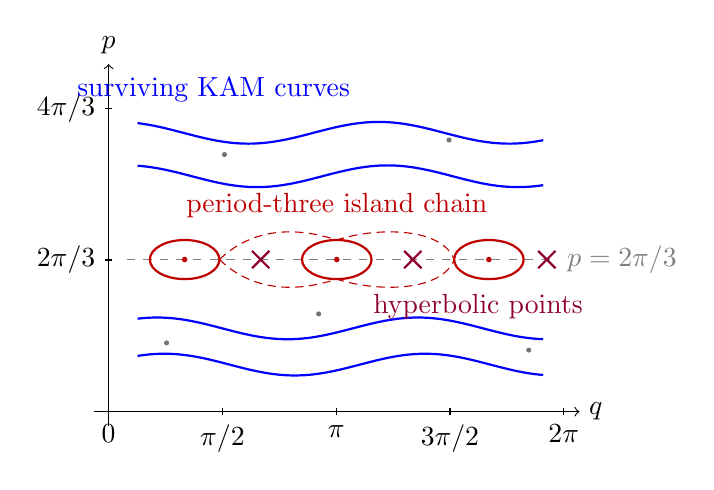
\begin{tikzpicture}[scale=0.92]
  \draw[->] (-0.2,0) -- (6.5,0) node[right] {\(q\)};
  \draw[->] (0,-0.2) -- (0,4.8) node[above] {\(p\)};
  \draw (0,0.05) -- (0,-0.05) node[below] {\(0\)};
  \draw (1.5708,0.05) -- (1.5708,-0.05) node[below] {\(\pi/2\)};
  \draw (3.1416,0.05) -- (3.1416,-0.05) node[below] {\(\pi\)};
  \draw (4.7124,0.05) -- (4.7124,-0.05) node[below] {\(3\pi/2\)};
  \draw (6.2832,0.05) -- (6.2832,-0.05) node[below] {\(2\pi\)};
  \draw (0.05,2.094) -- (-0.05,2.094) node[left] {\(2\pi/3\)};
  \draw (0.05,4.189) -- (-0.05,4.189) node[left] {\(4\pi/3\)};
  \foreach \y in {0.65,1.15,3.25,3.85}
    \draw[blue, thick, domain=0.4:6.0, samples=100]
      plot (\x,{\y+0.15*sin(100*\x+\y*20)});
  \draw[dashed, gray] (0.25,2.1) -- (6.2,2.1)
    node[right] {\(p=2\pi/3\)};
  \foreach \x in {1.05,3.15,5.25}
  {
    \draw[red!75!black, thick] (\x,2.1) ellipse (0.48 and 0.27);
    \fill[red!75!black] (\x,2.1) circle (1.1pt);
  }
  \draw[red!75!black, densely dashed]
    (1.53,2.1) .. controls (2.0,2.55) and (2.6,2.55) .. (3.15,2.37)
    .. controls (3.7,2.55) and (4.6,2.55) .. (4.77,2.1);
  \draw[red!75!black, densely dashed]
    (1.53,2.1) .. controls (2.0,1.65) and (2.6,1.65) .. (3.15,1.83)
    .. controls (3.7,1.65) and (4.6,1.65) .. (4.77,2.1);
  \foreach \x in {2.10,4.20,6.05}
  {
    \draw[purple!75!black, thick] (\x-0.12,1.98) -- (\x+0.12,2.22);
    \draw[purple!75!black, thick] (\x-0.12,2.22) -- (\x+0.12,1.98);
  }
  \foreach \x/\y in {0.8/0.95,1.6/3.55,2.9/1.35,4.7/3.75,5.8/0.85}
    \fill[black!55] (\x,\y) circle (1.0pt);
  \node[blue] at (1.45,4.45) {surviving KAM curves};
  \node[red!75!black] at (3.15,2.85) {period-three island chain};
  \node[purple!75!black] at (5.1,1.45) {hyperbolic points};
\end{tikzpicture}
\caption{Schematic phase portrait of an area-preserving map near a
period-three resonance: invariant curves, a chain of three islands, hyperbolic
points, and scattered chaotic points coexist.}
\label{fig:standard-map-island-chain}
\end{figure}

\section{Restricted Sun-Jupiter-Asteroid Equations}
\label{sec:restricted-sun-jupiter-asteroid}

Let \(r\in\R^2\) be the asteroid position relative to the Sun. Jupiter is
prescribed by
\[
  r_J(t)=a_J(\cos n_Jt,\sin n_Jt),
  \qquad
  n_J^2=\frac{G(M_\odot+M_J)}{a_J^3}.
\]
In a heliocentric non-inertial frame, the asteroid acceleration is
\[
  \boxed{
  \ddot r
  =
  -\frac{GM_\odot r}{\norm r^3}
  -
  GM_J
  \left(
    \frac{r-r_J}{\norm{r-r_J}^3}
    +
    \frac{r_J}{\norm{r_J}^3}
  \right)
  }.
\]
The first term is solar gravity. The first part of the Jupiter term is direct
gravitational attraction to Jupiter. The final term is the indirect term caused
by the acceleration of the heliocentric frame.

\begin{derivation}[Indirect term]
Let \(x\) be the asteroid position in an inertial frame and \(x_\odot\) the Sun
position. The heliocentric vector is \(r=x-x_\odot\). Then
\[
  \ddot r=\ddot x-\ddot x_\odot.
\]
The direct Jupiter acceleration of the asteroid is
\[
  -GM_J\frac{x-x_J}{\norm{x-x_J}^3}.
\]
The acceleration of the Sun due to Jupiter is
\[
  \ddot x_\odot=
  GM_J\frac{x_J-x_\odot}{\norm{x_J-x_\odot}^3}
  =
  GM_J\frac{r_J}{\norm{r_J}^3}.
\]
Subtracting \(\ddot x_\odot\) produces the indirect term
\[
  -GM_J\frac{r_J}{\norm{r_J}^3}.
\]
\end{derivation}

\section{Numerical Ejection Probability}
\label{sec:numerical-ejection-probability}

The highlighted simulation samples \(N\) test particles with initial semimajor
axes \(a_0\in[a_{\min},a_{\max}]\), small eccentricities, random orbital phases,
and random periapse directions. Let \(T\) be the integration horizon.

\begin{definition}[Finite-time ejection probability]
For a specified model, sampling distribution, time step, and ejection criterion,
the finite-time ejection probability estimate is
\[
  \widehat P_{\mathrm{ej}}(T)
  =
  \frac{1}{N}
  \sum_{i=1}^{N}\mathbf 1\{\text{particle \(i\) is ejected before time \(T\)}\}.
\]
\end{definition}

\begin{assumption}[Ejection criterion in the demo]
The Python demo counts a particle as ejected if it reaches a large heliocentric
radius or if its heliocentric two-body energy is positive after it has moved
outside Jupiter's orbital scale. It separately records close approaches to
Jupiter and collisions with the inner solar cutoff.
\end{assumption}

This probability is not an intrinsic number attached to nature. It depends on:
\[
  \text{model}+\text{initial ensemble}+\text{time horizon}
  +\text{numerical method}+\text{loss criterion}.
\]
That dependence should be reported, not hidden.

\section{Integrator Used In The Demo}
\label{sec:asteroid-integrator}

The demo uses a kick-drift-kick style update. If \(a(r,t)\) is the acceleration,
then
\[
\begin{aligned}
  v_{n+1/2} &= v_n+\frac{\Delta t}{2}a(r_n,t_n),\\
  r_{n+1} &= r_n+\Delta t\,v_{n+1/2},\\
  v_{n+1} &= v_{n+1/2}+\frac{\Delta t}{2}a(r_{n+1},t_{n+1}).
\end{aligned}
\]
Because Jupiter's position is explicitly time-dependent in the prescribed
circular model, the method is not exactly the same as a symplectic map for an
autonomous finite-dimensional Hamiltonian. It is still much better pedagogically
than an opaque black-box integrator because every force evaluation is visible.

\section{What To Take Forward}
\label{sec:perturbation-chaos-take-forward}

\begin{itemize}
\item Integrable systems are organized by invariant tori, not merely by closed
form solutions.
\item Resonance is a geometric condition \(k\cdot\omega=0\). It marks where
averaging fails and where perturbations can accumulate coherently.
\item Small divisors are not a technical nuisance; they are the arithmetic
trace of dense resonances.
\item KAM theory says that sufficiently irrational tori persist, but it also
highlights what is lost: resonant tori reorganize into island chains,
separatrices, and chaotic transport channels.
\item Numerical ejection probabilities are finite-time, model-dependent
observables. They become meaningful only when the sampling rule, integration
time, timestep, and loss criterion are stated.
\end{itemize}

\section{Questions For The Reader}
\label{sec:asteroid-reader-questions}

\begin{enumerate}
\item How does \(\widehat P_{\mathrm{ej}}(T)\) change with \(T\)?
\item Which semimajor-axis bins have the largest ejection fractions?
\item What changes when \(M_J\) is scaled upward?
\item Which losses are close encounters rather than clean ejections?
\item How sensitive are the results to \(\Delta t\)?
\item Are apparent resonance structures stable under a different random seed?
\end{enumerate}

\section{Associated Demos}
\label{sec:chaos-associated-demos}

\begin{itemize}
\item \path{demos/python/standard_map.py}
\item \path{demos/python/hamiltonian_pendulum.py}
\item \path{demos/python/asteroid_ejection_probability.py}
\item \path{demos/mathematica/AsteroidEjectionProbability.wl}
\end{itemize}
